\documentclass{article}
% --- Page Layout ---
\usepackage[a4paper, landscape, twocolumn, margin=1.5cm, columnsep=1cm]{geometry}
\usepackage[hidelinks]{hyperref}


% --- Text ---
\usepackage{ulem, multicol, afterpage, enumitem}
\let\oldemph\emph
\renewcommand{\emph}[1]{\textit{#1}}


% --- Code --- 
\usepackage{algpseudocodex}
\algrenewcommand\algorithmicforall{\textbf{for each}}


% --- Math ---
\usepackage{amsthm, amsmath, amsfonts, amssymb}
\numberwithin{equation}{section}
\usepackage{xcolor, tcolorbox}
\tcbuselibrary{theorems}


% --- Environments ---
\definecolor{darkgreen}{RGB}{19, 79, 25}

\newenvironment{pane}{
    \begin{tcolorbox}[left=5pt, right=5pt, center, colback=gray!5!white, colframe=gray!50]
}{
    \end{tcolorbox}
}

\newenvironment{myproof}[1]{
    \begin{tcolorbox}[colback=white, colframe=gray!50, title=\bfseries #1]
}{
    \end{tcolorbox}
}
\newenvironment{continueMyproof}{
    \begin{tcolorbox}[colback=white, colframe=gray!50]
}{
    \end{tcolorbox}
}

\newenvironment{definitions}{
    \begin{tcolorbox}[right=30pt, colback=darkgreen!9, colframe=darkgreen, title=\bfseries Definitions]
}{
    \end{tcolorbox}
}
\newenvironment{definition}[1]{
    \begin{tcolorbox}[colback=darkgreen!9, colframe=darkgreen, title=\bfseries Definition#1]
}{
    \end{tcolorbox}
}

\newenvironment{example}[1]{
    \begin{tcolorbox}[colback=blue!5!white, colframe=blue!75!black, title=\bfseries Example#1]
}{
    \end{tcolorbox}
}
\newenvironment{continueExample}{
    \begin{tcolorbox}[colback=blue!5!white, colframe=blue!75!black]
}{
    \end{tcolorbox}
}

\newenvironment{exercise}[1]{
    \begin{tcolorbox}[colback=white, colframe=gray!75!black, title=\bfseries Exercise#1]
}{
    \end{tcolorbox}
}
\newenvironment{continueExercise}{
    \begin{tcolorbox}[colback=white, colframe=gray!75!black]
}{
    \end{tcolorbox}
}


% --- Theorems & Definitions ---
%\renewcommand\qedsymbol{$\blacksquare$}
\newtcbtheorem{Definition}{Definition}
{colback=red!5!white, colframe=red!75!black, fonttitle=\bfseries}{}
\newtcbtheorem{Corollary}{Corollary}
{colback=purple!5!white, colframe=purple!80, fonttitle=\bfseries}{}
\newtcbtheorem{Theorem}{Theorem}
{colback=green!5!white, colframe=green!75!black, fonttitle=\bfseries}{}


% --- Graphics ---
\usepackage{graphicx}
\graphicspath{ {./images/} }
\usepackage{wrapfig}
\usepackage{tikz}

\author{Alessia Crimaldi}
\begin{document}
	\begin{titlepage}
    	\vspace*{\fill}
   		\centering
   		\Huge Languages and Algorithms for Artificial Intelligence\\
		\vspace{0.2cm}
   		\huge Module 3: Foundations, Computational Complexity, and Learning Theory\\
   		\vspace{0.7cm}
   		\Large Alessia Crimaldi
    	\vspace*{\fill}
	\end{titlepage}
	\pagenumbering{gobble}
	\tableofcontents
	\clearpage
	\pagenumbering{arabic}
	\parindent 0pt
	\cleardoublepage

	\section{Foundations}
		\subsection{Introduction}
			\paragraph{\large Is there any limit to what AI can do?}
			\mbox{}
			\vspace{0.1cm}
			
			This question arises from the awareness that AI is getting pervasive and it's used in many different fields.
			In this module, rather than asking what AI and ML can do and how we can exploit it, we'll try to give an answer to the question:
			\begin{center}
				\textit{``Is there any intrinsic limit to what we can do with AI and ML, or to the accuracy or efficiency of algorithms solving a given problem?"}
			\end{center}
			In other words, is there a problem which is impossible to be tractable by AI? And can computer scientists and engineers do everything with AI?
			\vspace{0.1cm}
			
			An example of a problem that AI is hardly able to solve is the Sudoku one, which is a backtracking algorithm and because of that it takes a huge amount of time: in principle we can solve the problem in 14 lines of code, but in practice the algorithm takes too much time. Other examples are \textit{NP complete problems}, that we will deepen.
			\paragraph{\large A paradigm shift.}
			\mbox{}
			\vspace{0.1cm}
	
			We impose limits to what we can compute, so we judge if a task is solvable or not.
			\begin{pane}
				\begin{center}
					\textit{``Algorithm $X$ (or Deep Learning model $X$) solves Problem $Y$\\ 
					efficiently and with great accuracy"}
				\end{center}
			\end{pane}
			E.g. Convolutional neural networks are so good in computer vision tasks.\\
			$X$: Convolutional neural network\\
			$Y$: Computer vision
			\begin{pane}
				$$\Downarrow{\text{derivation}_1: \text{\textbf{Computability}}}$$
				\begin{center}
					\textit{``Problem $Y$ cannot be solved by any Algorithm $X$"}
				\end{center}
			\end{pane}
			This is a very strong statement: it means that there is no code to solve the problem $Y$ whatsoever. So problem $Y$ is kinda \uline{unsolvable}.
			\begin{pane}
				$$\Downarrow{\text{derivation}_2: \text{\textbf{Complexity}}}$$
				\begin{center}
					\textit{``Any Algorithm solving $Y$ is bound to be inefficient, or not accurate"}
				\end{center}
			\end{pane}
			If we prove derivation$_1$, then any attempt to solve problem $Y$ would be useless. But if instead derivation$_1$ fails, we can try proving derivation$_2$, which states that any problem $Y$ can be solved by an algorithm, but it can't be solved in a reasonable amount of time or with a reasonable amount of computational resources (e.g. Sudoku).
			\vspace{0.2cm}
			
			Representing the space of all possible problems we are interested in solving, there's a huge class of problems that are meaningful, although there are even problems outside of this set, which are so difficult and so hard even to describe.\\
			\begin{wrapfigure}{l}{0.45\linewidth}
				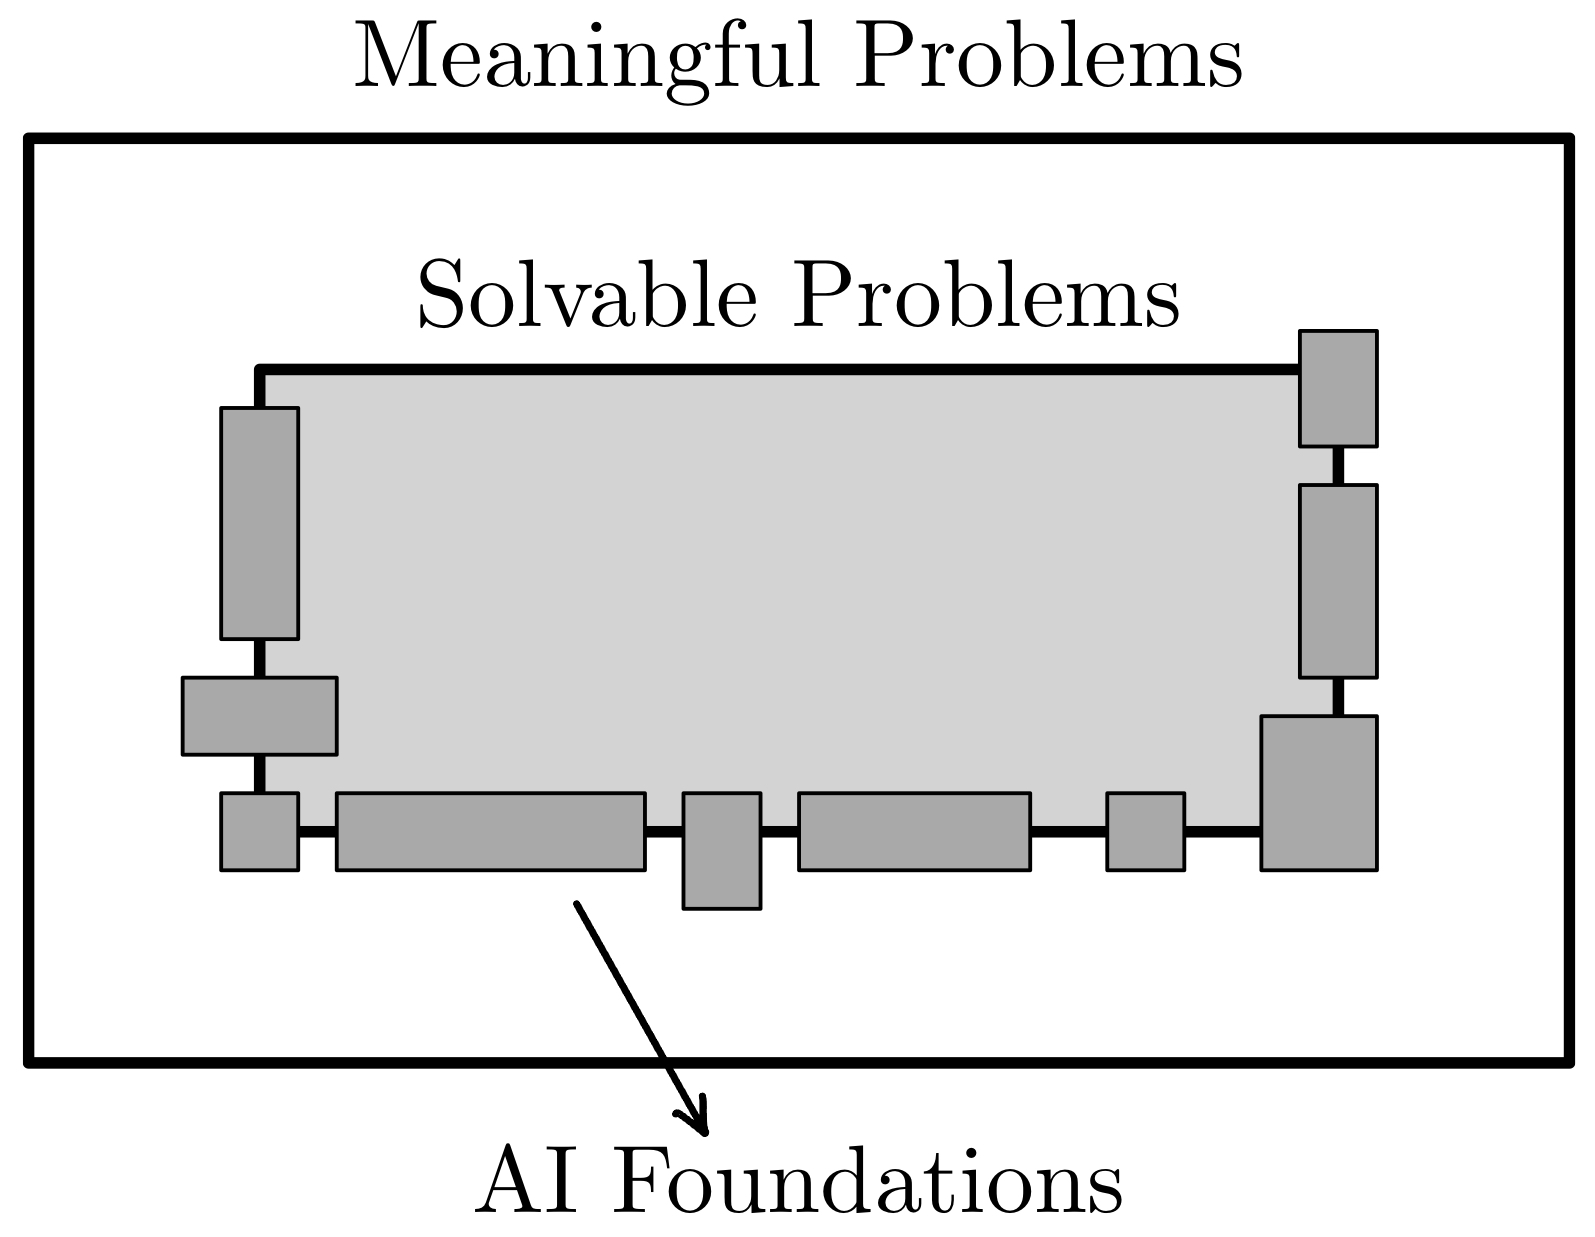
\includegraphics[width=1\linewidth]{space_of_problems}
			\end{wrapfigure}
			\textbf{Meaningful Problems:} problems which can at least be described in a formal way, without too many ambiguities.\\\\
			\textbf{Solvable Problems:} A rather small class, which contains problems for which there is a process, which is able to solve any instance of the given problem with a reasonable degree of accuracy and within a reasonable amount of time.\\\\
			\textbf{AI Applications} are many and scattered within these two sets, but in this module we will focus on \textbf{AI Foundations} and what's at the borders of the \textit{Solvable Problems}.
			\paragraph{\large The value of negative results.}
			\mbox{}
			\vspace{0.1cm}
			
			\begin{pane}
				\centering
				\textit{``Negative results are just what I want. They're just as valuable to me as positive results. I can never find the thing that does the job best until}\\
				\textit{I find the ones that don't."}\\
				\raggedleft
				{\small - Thomas A. Edison}
			\end{pane}
			This quote is important because if we know that the task we want to accomplish is intrinsically \emph{hard}, and we know \emph{in what} its hardness resides, we can:
			\begin{enumerate}
				\item Direct our work towards methodologies \textit{specifically designed} for hard tasks.
				\vspace{-0.25cm}
				\item \textit{Avoid} spending our time trying to design solutions that cannot exist.
				\vspace{-0.25cm}
				\item Inform the stakeholders \textit{in advance} that the solution we are going to design will likely be inefficient.
				\vspace{-0.25cm}
				\item Decide that the task is \textit{too difficult}, and that it cannot be accomplished the way we want.
				\vspace{-0.25cm}
				\item Decide that it is better to switch to a \textit{relaxed} version of the task, which instead admits reasonable solutions.
			\end{enumerate}
		\subsection{Historical, Conceptual, and Mathematical Preliminaries}
			\paragraph{\large Computability and Complexity.}
			\mbox{}
			\begin{definition}{: Theory of Computation}
				\textit{Theory of Computation} (aka \textbf{ToC}) is a branch of theoretical computer science that explores the fundamental capabilities and limitations of computers, including what can be computed and how efficiently. Specifically, it investigates whether and how problems can be solved using algorithms and models of computation.
			\end{definition}
			Until the late 60s, ToC was mainly concerned with understanding \textbf{computability:}
			\begin{definition}{: Computability Theory}
				\texttt{Main Question:} is a certain task computable?
				\vspace{0.2cm}
				
				If the answer is negative, the task is said to be \uline{\textit{uncomputable}} (and there can be many ways in which this can happen).
			\end{definition}
			\vspace{0.1cm}
			
			Then, at the end of the 60s, a paradigm shift\footnote{The paradigm shift was from Computability Theory to Computational Complexity Theory.} happened. Indeed, since the pioneering works by Hartmanis, Stearns, and Cobham (all from the late 60s), a new branch of ToC has emerged, which deals with \textbf{efficiency:}
			\begin{definition}{: Computational Complexity Theory}
				\texttt{Main Question:} is a certain task solvable in a reasonable amount of time, or space (i.e. working memory)?
				\vspace{0.2cm}
				
				If the answer is negative, the task is maybe computable, but requires so much time or space, that is becomes \uline{\textit{practically uncomputable}}.
			\end{definition}
			In \textbf{Computational Complexity Theory}, we rarely succeed in proving the nonexistence of an efficient algorithm. Instead, the field focuses on comparing the difficulty of different problems, rather than categorising them as absolutely hard or easy.
			\vspace{0.15cm}
			
			Some central research questions in CCT are:
			\vspace{-0.1cm}
			\begin{itemize}
				\item Can the use of randomness help speed up computation?
				\vspace{-0.25cm}
				\item Can hard tasks become easier if we allow algorithms to make occasional errors on a relatively small subset of the inputs?
				\vspace{-0.25cm}
				\item Can we exploit the hardness of certain tasks?
				\vspace{-0.25cm}
				\item Can we make use of some counterintuitive properties of quantum mechanics to build faster computing devices?
				\vspace{-0.25cm}
				\item The \textbf{P} vs. \textbf{NP} question.
			\end{itemize}
			\newpage
			\paragraph{\large Modeling computation.}
			\mbox{}
			\vspace{0.1cm}
			
			The Standard Paradigm:
			\begin{center}
    			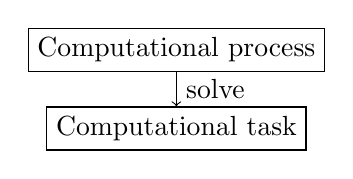
\begin{tikzpicture}
        			\node[draw, rectangle] (process) {Computational process};
        			\node[draw, rectangle, below of=process] (task) {Computational task};
        			\draw[->] (process) -- (task) node[midway, right] {solve};
    			\end{tikzpicture}
    			\vspace{0.15cm}
			\end{center}
			We employ a \textbf{computational process} (\textit{how}), such as a program, algorithm, or machine learning model, to \textit{solve} specific \textbf{computational tasks} (\textit{what}), representing problems that we aim to solve.
			\vspace{0.1cm}
			
			There can be an infinite amount of processes that solve a specified task. On the other hand, some tasks are so difficult that no existing process can solve them.
			\vspace{0.1cm}
			
			In the Theory of Computation a process can be viewed as an \textbf{algorithm} or a Python program that doesn't use any external library. This algorithm must satisfy the following constraints:
			\begin{itemize}
    			\item It should consist of a finite series of steps;
    			\item Each of these steps need to be elementary;
    			\item The way the next step is determined must be deterministic, offering an unambiguous instructions that transit from one state to another.
			\end{itemize}
			\begin{example}{: Multiplication Problem}
				{\small
				\paragraph{\small Problem (natural number multiplication).}
				Suppose you want to write a Python program which multiplies two positive integer numbers, which can both be expressed as $n$-digits numbers, but which are represented as lists rather than scalars.
				Suppose that the operations at your disposal are just the basic arithmetic operations \textit{on digits}, so that you cannot just multiply the two numbers.
				How should you write your program?\\
				\paragraph{\small Task.}
				Multiplying two natural numbers $a$ and $b$ both expressible with $n$ digits, by performing operations on digits.\\
				\paragraph{\small Solution.}
				Suppose we have the two lists with $n = 4$ number of digits:\\
				\begin{center}
					1: \BoxedString{3} \BoxedString{2} \BoxedString{5} \BoxedString{1}\\
					2: \BoxedString{2} \BoxedString{1} \BoxedString{7} \BoxedString{2}
				\end{center}
				We want to compute the list which stands for the product of the two lists, and there are different processes which can solve this same task.
				}
			\end{example}
			\begin{continueExample}
				{\small
				\begin{enumerate}[leftmargin=*]
					\item \texttt{RepeatedAddition:} a process solving the task above that consists in reducing multiplication to addition:
					$$a \cdot b = \underbrace{a + a + \dots + a}_{b\;\text{times}}$$
					This simple algorithm sums the first number with itself a number of times equal to the second number: multiplication is repeated addition.
					\vspace{0.1cm}
					
					Since addition of two $n$-digit numbers is a relatively easy process which can be carried out in a linear amount of steps, the total number of steps is proportional to $\mathbf{b \cdot n}$.
					\item \texttt{GridMethod:} another process solving the task above that consists in rather multiplying $a$ and $b$ with the elementary school direct algorithm:
					\begin{center}
						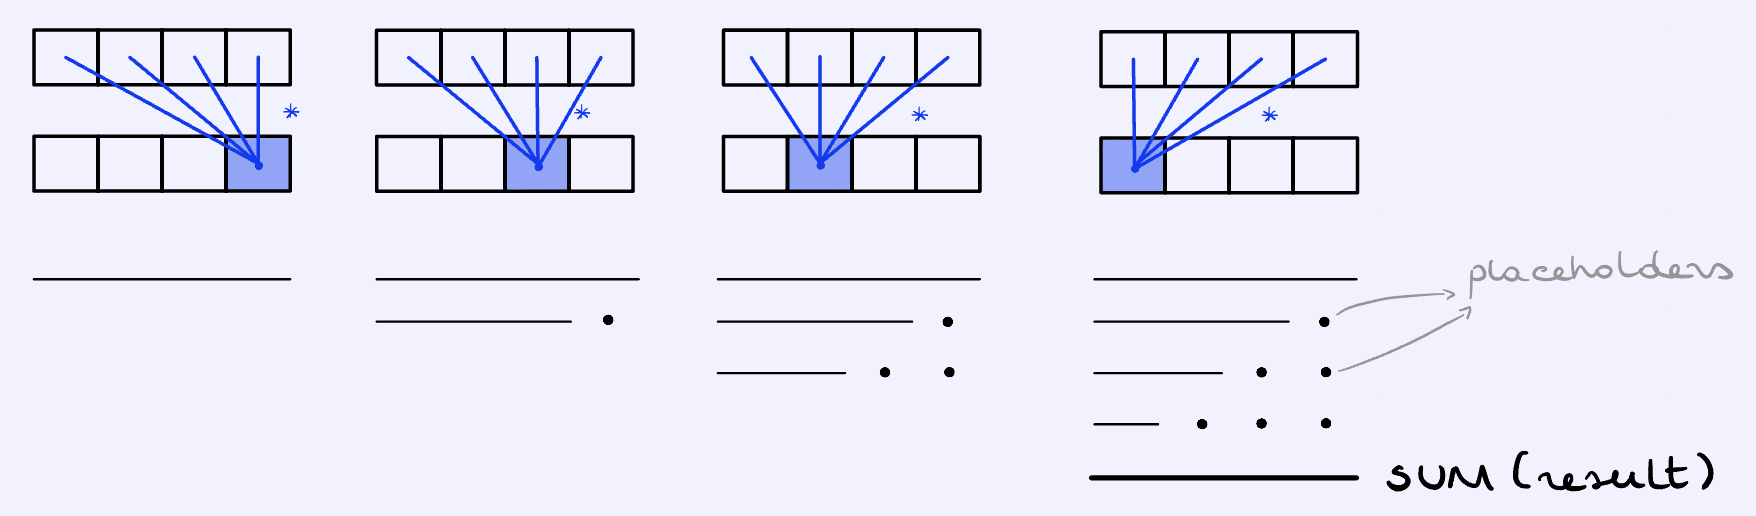
\includegraphics[width=0.85\linewidth]{natural_number_multiplication}
					\end{center}	
					It takes an amount of steps which is proportional to $\mathbf{n \cdot n}$.
				\end{enumerate}
				\vspace{0.3cm}
				\paragraph{\small Are they equivalent or not?}
				They're not equivalent. There is an exponential difference between the performances of \texttt{RepeatedAddition} and \texttt{GridMethod}: $b$ can be exponential in $n$ in the number of digits, at most $10^n - 1$.
				\paragraph{\small Which one is the best?}
				The \texttt{GridMethod} is better. There is a huge different if we take $100$ digits: if each basic instruction takes a millisecond, \texttt{GridMethod} would take one second, while \texttt{RepeatedAddition} would take more than $10^{80}$ years.
				\begin{center}
    				\begin{tabular}{c|c|c|c}
    					& \textbf{Time} & \textbf{Complexity} & \textbf{Class}\\
    					\hline
        				\texttt{GridMethod} & $100*100$ & polynomial time & P\\
        				\hline
        				\texttt{RepeatedAddition} & $(10^{100} - 1) * 100$ & exponential time & EXP\\
    				\end{tabular}
    			\end{center}
    			\vspace{0.2cm}
    			$\blacktriangleright$ Distinct processes can solve the same task in very different ways, and not all of them are acceptable.\\
    			$\blacktriangleright$ \texttt{GridMethod} witnesses the fact that the task is in a class of tasks called \textbf{P}.
    			}
			\end{continueExample}
			\begin{example}{: Wedding Problem}
				{\small
				\paragraph{\small Problem (maximum independent set).}
				Suppose you are going to marry your boyfriend (or girlfriend) soon and you want to decide the list of invitees. Since your soon-to-be father-in-law will pay all bill, you have all the interest in keeping the list of invitees as large as possible. But actually, it would be impossible to invite all the people in the set $L = \{ a_1, \dots, a_n \}$ of all candidate invitees since some of them are kind of incompatible and cannot be invited together; i.e. there is another set $I = \{ (b_1, c_1), \dots, (b_n, c_n) \} \subseteq L \times L$ whose elements are those candiate invitees pairs which are incompatible. Would it be possible to maximise the length of the list of invitees?\\
				\paragraph{\small Task.}
				Given a set $L$ of candidate invitees, and a list $I \subseteq L \times L$ of incompatible pairs of candidate invitees, find the largest subset of $L$ composed of compatible invitees.\\
				\paragraph{\small Solution.}
					A process solving the task consists in considering all possible subsets of the set $L$ (\emph{brute force}), check each for the presence of incompatibilities, and track their sizes. However, if $L$ contains $n$ elements, then it has $2^n$ different subsets, which is impractical. This exponential growth makes the problem computationally expensive.\\
					
				$\blacktriangleright$ This is an optimisation problem, but the decisional version of this problem is known to belong to the \textbf{class NP}.\\
				$\blacktriangleright$ The real question is \emph{Can we do better} than exhaustive enumeration? It remains unclear whether NP problems can be solved more efficiently.\\
				$\blacktriangleright$ If we were to find a significantly better solution, we would effectively resolve the long-standing question of whether \textbf{NP $=$ P}.
				}
			\end{example}
			\begin{example}{: Learning programs with finite inputs and outputs}
				{\small
				\paragraph{\small Problem.}
				Suppose your ML teacher asks you to write a learning algorithm capable of reconstructing a program by querying it as a black box, without looking at the code. You can assume that the program takes in input a list of booleans of a fixed (rather big) length $n$, and produces in output one boolean value. How would you proceed? On which input would you query the program? Would it be possible to query the program on significantly less inputs than the $2^n$ possible ones?\\
				\paragraph{\small Solution.}
				No, if we do not know anything about the program, we have to query it as a black box on all $2^n$ possible inputs. And if $n$ becomes bigger, this number of possible inputs gets completely intractable and out of reach even when $n$ is not so big (e.g. 300). On the contrary, in the case in which we know that the program has a certain shape, then we can do something.
				}
			\end{example}
			\paragraph{\large Mathematical Preliminaries.}
			\paragraph{Sets and numbers.}
			\begin{itemize}
   				\item We focus on numbers $x$ that belongs either to the set of natural numbers $\mathbb{N}$ or to the set of integers $\mathbb{Z}$.
    			\item The cardinality of any given set $X$ is denoted by $\left\lvert X\right\rvert$. It can be finite or infinite, but not uncountable.
    			\item When we refer to a logarithm of a number $\log x$, we imply the base 2 logarithm.
    			\item For a given real number $x$, $\lceil x \rceil$ is the smallest element of $\mathbb{Z}$ such that $\lceil x \rceil \geq x$. Whenever a real number $x$ is used in place of a natural number, we implicitly read it as $\lceil x \rceil$.
    			\item For a natural number $n$, $[n]$ is the set $\{1,\dots,n\}$.
    			\item We say that a condition $P(n)$ holds for \uline{sufficiently large} $n\in \mathbb{N}$ if there exists an $N\in \mathbb{N}$ such that $P(n)$ holds for every $n>N$.
			\end{itemize}
			\paragraph{Strings.}
			\mbox{}
			\vspace{0.1cm}
	
			Given an alphabet $S$, which is a finite set of symbols, a \textbf{\textit{string}} is defined as a finite, ordered, possibly empty sequence of elements selected from $S$. We categorise sets of strings based on their lengths as follows:
			\begin{itemize}
    			\item $S^0$: is the set containing only the empty string, denoted as $\epsilon$.
    			\item $S^n$: is the set of all strings over $S$ of length exactly $n\in\mathbb{N}$.
    			\item $S^*$: is the set of all strings over $S$ and is $\bigcup_{n=0}^\infty S^n$.
			\end{itemize}
			The \textbf{concatenation} of two strings $x$ and $y$ over $S$ is indicated as $xy$ or as $x\cdot y$. The string over $S$ obtained by concatenating $x$ with itself $k\in \mathbb{N}$ times is indicated as $x^k$.\\
			The set of all strings over $S$, together with the concatenation operation, forms a \textbf{\textit{monoid}}. A monoid is an algebraic structure consisting of an associative binary operation (in this case, string concatenation) and an identity element (the empty string $\epsilon$, since concatenating it with any string leaves the string unchanged).\\
			The \textbf{length} of a string $x$ is indicated as $\left\lvert x\right\rvert$.
			\vspace{0.1cm}
			\begin{example}{: $S^n$ and length of a string}
    			$$\{0,1\}^2=\{00,01,10,11\}\qquad \left\lvert 000101\right\rvert=6$$
			\end{example}
			\paragraph{Tasks as functions.}
			\mbox{}
			\vspace{0.1cm}
	
			Most tasks consist of turning an input into an output, so they can be viewed as computing a function from $\{0,1\}^*$ to $\{0,1\}^*$. Then, we always assume that the task we want to solve is given as a function $f: A \rightarrow B$ where both the domain $A$ and $B$ are discrete (i.e. countable) sets, sometimes leaving the encoding of $A$ and $B$ into $\{0,1\}^*$ implicit.
			\vspace{0.15cm}
			
			When the input and/or outputs are not binary strings but originate from discrete sets, they can be encoded as binary strings following some encoding. The encoding of any element $x$ of $A$ as a string is often indicated as $\llcorner x \lrcorner$ or simply as $x$.
			\vspace{0.1cm}
			\begin{example}{: Enconding objects as strings}
    			\begin{itemize}[leftmargin=*]
        			\item Strings in $S^*$, where $S=\{a,b,c\}$:
            			\begin{itemize}
                			\item $a\mapsto00,\ b\mapsto 01,\ c\mapsto 10$
                			\item $abbc\mapsto 00010110$
            			\end{itemize}
        			\item Natural numbers:
        			\begin{itemize}
        				\item $12\mapsto 1100$	
        			\end{itemize}
        			\item Pairs of binary strings, i.e. $\{0,1\}^* \times \{0,1\}^*$:
        				\begin{itemize}
        					\item $(x,y)\mapsto x\#y$ (over the alphabet $\{0,1,\#\}$), then encode it as before.
        					\item $(011, 100) \mapsto 011\#100 \mapsto \underbrace{00}_{0} \; \underbrace{01}_{1} \; \underbrace{01}_{1} \; \underbrace{10}_{\#} \; \underbrace{01}_{1} \; \underbrace{00}_{0} \; \underbrace{00}_{0}$
        				\end{itemize}
    			\end{itemize}
			\end{example}
			\paragraph{Languages and Decision Problems.}
			\mbox{}
			\vspace{0.1cm}
			
			Very often the functions from $\{0,1\}^*$ to $\{0,1\}^*$ we are interested in studying as tasks are functions from binary strings to peaks, i.e. they return either 0 or 1. These are the so called \textbf{\textit{boolean functions}} (aka \textit{characteristic functions}), or simply \textbf{\textit{languages}}.
			\begin{definition}{: Boolean function or ``language"}
				A function from $\{0,1\}^*$ to $\{0,1\}$, that is, it maps binary strings of arbitrary length to a single bit (0 or 1). Such a function $f$ is identified with the subset $\mathcal{L}_f$ of $\{0,1\}^*$:
				$$\mathcal{L}_f = \{x \in \{0,1\}^* \; \vert \; f(x) = 1\}$$
			\end{definition}
			This subset $\mathcal{L}_f$ is referred to as a language. More generally, any subset of $S^*$ (the set of all strings over an alphabet $S$) is usually called a \textbf{language}.\\
			This way, a \textbf{decision problem} for a given language $\mathcal{M}$ (i.e. is $x \in \{0,1\}^*$ in $\mathcal{M}$?) can be seen as the task of computing $f$ such that $\mathcal{M}=\mathcal{L}_f$.
			\begin{definition}{: Decision problem}
				Special kind of problem which corresponds to deciding whether a given string (i.e. a binary string) belongs to a particular language (i.e. a given subset of a set of binary strings).
			\end{definition}
			\paragraph{Asymptotic notation.}
			\mbox{}
			\vspace{0.1cm}

			We can study in which relation two functions
			$f$ and $g$ are by studying the limit of $\frac{f(n)}{g(n)}$ for $n\to\infty$:
			\begin{itemize}
    			\item A function $f: \mathbb{N} \rightarrow \mathbb{N}$ is $O(g)$ if there is a positive real constant \(c\) such that \(f(n) \leq c \cdot g(n)\) for sufficiently large $n$.
        			\begin{itemize}
            			\item \texttt{Example:} the function $n \mapsto 3n^2 + 4n\) is \(O(n^2)\), but also \(O(n^3)\), and certainly \(O(2^n)$. It is not, however, $O(n)$.
        			\end{itemize}
    			\item A function $f: \mathbb{N} \rightarrow \mathbb{N}$ is $\Omega(g)$ if there is a positive real constant $c$ such that $f(n) \geq c \cdot g(n)$ for sufficiently large $n$.
        			\begin{itemize}
            			\item \texttt{Example:} the function $n \mapsto 3n^2 + 4n$ is $\Omega(n^2)$, but also \(\Omega(n)\), but not $\Omega(n^3)$.
        			\end{itemize}
    			\item A function $f$ is $\Theta(g)$ if $f$ is both $O(g)$ and $\Omega(g)$.
        			\begin{itemize}
            			\item \texttt{Example:} the function $n \mapsto 3n^2 + 4n + 7$ is $\Theta(n^2)$.
        			\end{itemize}
			\end{itemize}
		\subsection{Exercises on the Mathematical Preliminaries}
			Here are some exercises focusing on sets, induction, cardinality and natural numbers.\\
			\begin{pane}
				\paragraph{Proving by induction.}
				We want to prove that a given property  holds when $n=0$ and also holds for $n+1$, provided it holds for $n$. So, an induction proof always follows that structured approach:
				\begin{itemize}
					\item \uline{\textit{Base case}:} we first establish the validity of the given property for the base case, often \uline{$n=0$}.
					\item \uline{\textit{Inductive case}:} then we demonstrate that if the property holds for an arbitrary $n$, it must also hold for \uline{$n+1$}.
				\end{itemize}
			\end{pane}
			\begin{exercise}{ 1: Induction on natural numbers}
				\paragraph{Problem.}
				What is the cardinality of $S^n$, namely the set of all strings of length $n$ in the alphabet $S$? Prove your claim.\\
				\paragraph{Solution.}
				\mbox{}
				\vspace{0.1cm}
				
				$\left\lvert S^n\right\rvert=\left\lvert S\right\rvert^n$ $\Rightarrow$ The power operator commutes with the cardinality operator: it indicates that when raising a set of strings to a power within the cardinality operator, the power operation can be equivalently be applied to the cardinality operator itself.
				\vspace{0.15cm}
				
				\begin{proof}
					This can be proved by induction on the natural numbers.
					\begin{itemize}
    					\item \uline{\textit{Base case}:}
    					$$|S^0|=|\{\epsilon\}|=1=|S|^0$$
    					\item \uline{\textit{Inductive case}:} we have to derive $\left\lvert S^{n+1}\right\rvert= \left\lvert S\right\rvert^{n+1}$ from $\left\lvert S^n\right\rvert= \left\lvert S\right\rvert^n$. The trick here is to express $\left\lvert S^{n+1}\right\rvert$ in a form as close as possible to the form of the starting hypothesis:
        				$$\left\lvert S^{n+1}\right\rvert = \left\lvert S\cdot S^n\right\rvert$$
        				where the ``multiplication" of two set of strings $S \cdot S^n$ is the set of concatenated strings.\\
        				Also, when we multiply a set containing $k$ strings by another set containing $h$ strings, the total number of products is $k*h$. Thus, the cardinality of the product of two sets can be rewritten as:
        				$$=\left\lvert S\right\rvert \left\lvert S^n\right\rvert$$
        				Leveraging our original hypothesis, $\left\lvert S^n\right\rvert=\left\lvert S\right\rvert^n$, we substitute:
        				$$=\left\lvert S\right\rvert \left\lvert S\right\rvert^n$$
        				\begin{equation*}
							=\left\lvert S\right\rvert^{n+1} \qedhere
						\end{equation*}
					\end{itemize} 
				\end{proof}
			\end{exercise}
			\begin{exercise}{ 2: Induction on natural numbers}
				\paragraph{Problem.}
				Prove by induction on $n$ that $\sum^n_{i=1} \frac{n(n+1)}{2}$.
			\end{exercise}
			\begin{exercise}{ 3: Induction on strings}
				The reverse $x^R$ of a string $x$ is defined recursively as follows:
    			\begin{itemize}[leftmargin=*]
        			\item \textit{base case}: if $x=\epsilon$, then $x^{R}=\epsilon$
        			\item \textit{recursive case}: if $x=s\cdot y$ (where $s$ is a single character), then $x^R=y^R\cdot s$
    			\end{itemize}
    			\noindent\rule{\linewidth}{0.6pt}\vspace{-0.3cm}
    			\paragraph{Problem.}
				Prove that for every pair of strings $x,y$ it holds that $(x\cdot y)^R=y^R \cdot x^R$.
				\paragraph{Solution.}
				\begin{proof}
					We do the proof by induction on $\left\lvert x\right\rvert$:
					\begin{itemize}
        				\item \uline{\textit{Base case}:} $|x|=0\Rightarrow x=\epsilon$, then 
            			$$(x \cdot y)^R=(\epsilon \cdot y)^R = y^R = y^R \cdot \epsilon^R = y^R \cdot x^R$$
        				\item \uline{\textit{Inductive case}:} $|x|>0\Rightarrow x=s \cdot z$ (we can rewrite it as a character $s$ and the rest of the string $z$, because the string has at least 1 character), then
            			$$(x \cdot y)^R=((s \cdot z) \cdot y)^R$$
            			Using the associativity property of concatenation:
            			$$=(s\cdot(z\cdot y))^R$$
            			Applying the definition of the reverse of a string:
            			$$=(z\cdot y)^R\cdot s$$
            			Using the statement we want to prove as hypothesis:
            			$$=(y^R \cdot z^R) \cdot s$$
            			Using the associativity property of concatenation:
            			$$y^R \cdot (z^R \cdot s)$$
            			Applying the definition of the reverse of a string:
            			$$=y^R \cdot (s \cdot z)^R$$
            			\begin{equation*}
							=y^R \cdot x^R \qedhere
						\end{equation*}
    				\end{itemize}
    			\end{proof}
			\end{exercise}
			
		
		
		
		
		
		
		
		
		
		
		
		
		
		
		
		
		
		
		
		
		
		
		
		
	\cleardoublepage
	\section{Computability Theory}
		\subsection{The Computational Model}
		\subsection{Exercises about the Computational Model}
		\subsection{Exercises}

	\cleardoublepage
	\section{Computational Complexity}
		\subsection{Polynomial Time Computable Problems}
		\subsection{Exercises on Polynomial Time Computable Problems}
		\subsection{Exercises and Proofs on Exponential Time Computable Problems}
		\subsection{Between the Feasible and the Unfeasible}
		\subsection{Proofs about NP}
		\subsection{Proofs and Examples about NP}
		\subsection{Exercises}

	\cleardoublepage
	\section{Computational Learning Theory}
		\subsection{A Glimpse of Computational Learning Theory}
		\subsection{Proofs on Computational Learning Theory}
		\subsection{Exercises}


%%%%%%%%%%%%%%%%%%%%%%%%%%%%%%%%%%%%%%%%%%%%%%%%%%%%%%%%%%%%%%%%%%%%%%%%%%%%%%%%%
% Lecture 7 - 11.03.24
\begin{comment}
   		\begin{exercise}
			\paragraph{Problem.} Prove that the wedding plan problem as we have described it at the beginning of this module is in the class \textit{fexp}.\\
			\paragraph{Solution.} First of all, let us recall how the problem is defined. Given a list of invitees and a list of incompatibility constraints between invitees, we want to build a sublist of invitees which are compatible with each other, and which has maximal length.
			\begin{itemize}
				\item Let us then show how this problem is an instance of a more general problem about graphs, e.g.:
	    		\begin{center}
    				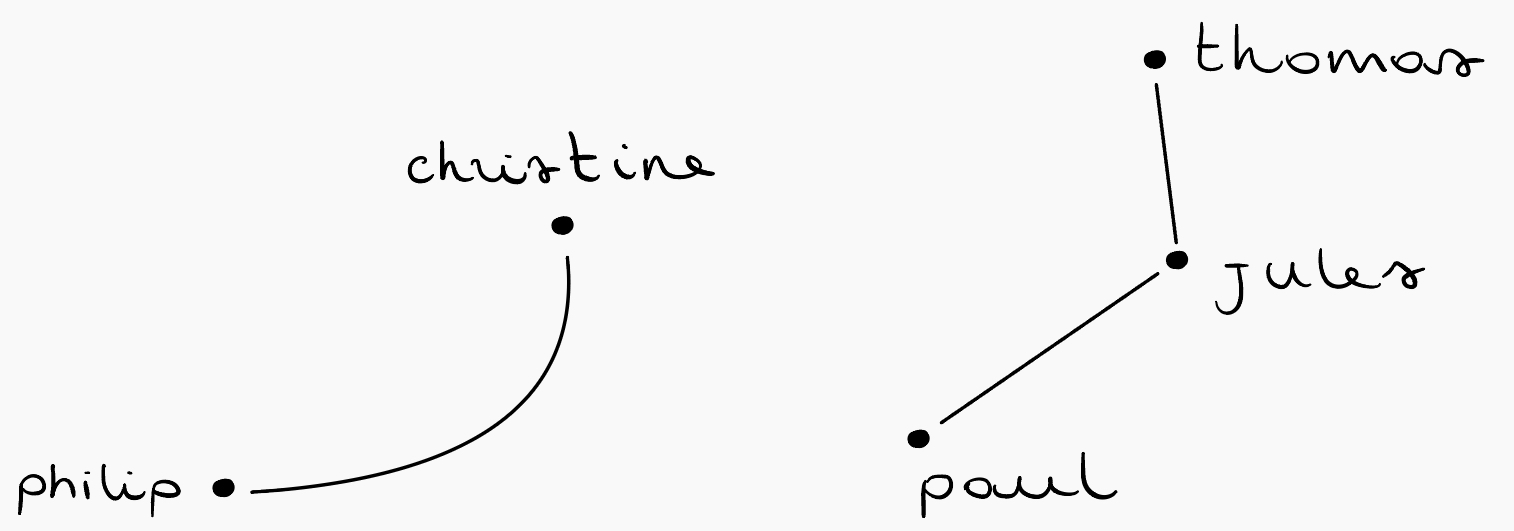
\includegraphics[width=0.65\linewidth]{graph_names_example}
				\end{center}
				$\mathbb{G} = (\{$philip, christine, paul, jules, thomas\}, \{\{philip, christine\}, \{paul, jules\}, \{jules, thomas\}\}\\
				$\mathbb{G}$ is an example of an \uline{undirected graph}, namely a pair $(V,E)$, where $V$ is as usual a set of nodes, while $E$ is a subset of $\{\{l, r\} \; | \; l, r \in V, l \neq r\}$.
				\item The wedding problem, then, can be spelled out as follows as a problem on undirected graphs: given $\mathbb{G} = (V,E)$ undirected graph, determine a subset of $V$, called $W$, satisfying the two conditions below:
				\begin{itemize}
					\item[i.] For all $v \in W, N(v) \wedge W = \emptyset$, where\\
		    		$N(v) = \{w \; | \; \{v, w\} \in V \} \subseteq V$\\
		    		(such a $w$ is called an \uline{independent set})
		    		\item[ii.] $|w|$, namely the number of nodes in $w$, is maximal among that of all subsets of $V$ satisfying $i$).
				\end{itemize}
				\item The function we want to prove in \textit{fexp}, then, is a function $maxindset$: 
				\begin{center}
					$graphs \; \rightarrow \; setsofnodes$
				\end{center}
				\begin{itemize}
	    			\item $graphs$: easily represented as a string
	    			\item $setsofnodes$: can be represented as a string in which 0 stands for $\notin$ and 1 stands for $\in$. $\lfloor \{$christine, paul$\} \rfloor$ = 01100.
	    		\end{itemize}
			\end{itemize}
		\end{exercise}
		\begin{continueExercise}
			\begin{itemize}
				\item The algorithm we are looking for, then looks as follows:
	    		\begin{itemize}
	    			\item input: an undirected graph G=(V,E)
	    			\item output: a subset $w \subseteq V$ (satisfying i and ii above).
	    		\end{itemize}
	    		\begin{algorithmic}
	    			\State $Z \leftarrow \emptyset$ \Comment{$1$}
	    			\For{\textbf{each} $W \subseteq V$} \Comment{$O(2^{|V|})$}
	    				\State ind $\leftarrow$ true \Comment{$1$}
	    				\ForAll{$w \in W$} \Comment{$O(|V|)$}
	    					\If{$N(w) \cap W \neq \emptyset$} \Comment{$2$}
	    						\State ind $\leftarrow$ false
	    					\EndIf
						\EndFor
						\If{ind} \Comment{$3$}
							\If{$|Z| < |W|$}
								\State Z $\leftarrow$ W
							\EndIf
						\EndIf
	    			\EndFor
	    			\State return z \Comment{$1$}
	    		\end{algorithmic}
			\end{itemize}
			\paragraph{Number of instructions.} An upper  bound on the number of instructions executed is:
			$$2 + O(2^{|v|})(4 + O(|v|) \cdot 2) =$$
			$$2 + O(2^{|v|}) \cdot O(|v|) \in O(2^{|v|^2})$$
			\paragraph{Size of intermediate results.} It is easily seen to be bounded by $O(|v|)$.
			\paragraph{Instructions we use as subroutines.} All the subroutines we use work in polynomial time.
		\end{continueExercise}
\end{comment}


%%%%%%%%%%%%%%%%%%%%%%%%%%%%%%%%%%%%%%%%%%%%%%%%%%%%%%%%%%%%%%%%%%%%%%%%%%%%%%%%%
% Lecture 8 - 12.03.24 (Exercitation)
\begin{comment}
		\clearpage
		\section{Exercises}
		\subsection{Turing Machines}
		
   		\begin{exercise}{ 3}
   			\paragraph{Problem.} Define a Turing machine computing the successor of a nonnegative integer in binary.\\
   			
   			\paragraph{Solution.}
   			\mbox{}
   			
   			integer $n \geq 0$ encoded in binary $w \in 10,15*$\\
   			\begin{enumerate}
   				\item there is a 0 in $w succ(1001) = 1010$
   				\item there is a 1 in $w$ succ(...) = ...
   			\end{enumerate}
   			\begin{itemize}
   				\item set of states $\mathbb{Q} = \{q_{init}, q_{halt}, $
   				\item transition function $\delta: \mathbb{Q} \times \Gamma^2 \rightarrow \mathbb{Q} \times \Gamma \times \{L,R\}$\\
   				
   				$(q_{first}, (1, 0)) \longmapsto (q_{halt}, 1, (S,S))$\\
   				$(q_{first}, (0, 0)) \longmapsto (q_{halt}, \square, (S,S))$\\
   				$(q_{ro}, (1, \square)) \longmapsto (q_{ro}, \square, (R,R))$\\
   				$(q_{ro}, (0, \square)) \longmapsto (q_{ro}, \square, (R,R))$\\
   				$(q_{ro}, (\square, \square)) \longmapsto (q_{l_1}, \square, (L,L))$\\
				$(q_{l_1}, (1, \square)) \longmapsto (q_{l_1}, 0, (L,L))$\\
				$(q_{l_1}, (0, \square)) \longmapsto (q_{l_0}, 1, (L,L))$\\
				$(q_{l_0}, (1, \square)) \longmapsto (q_{l_0}, 1, (L,L))$\\
				$(q_{l_0}, (0, \square)) \longmapsto (q_{l_0}, 0, (L,L))$\\
				$(q_{l_0}, (\rhd, \rhd)) \longmapsto (q_{halt}, \rhd, (S,S))$\\
   			\end{itemize}
   		\end{exercise}
   		
   		
   		\subsection{Rice's theorem}
   		
   		\begin{exercise}{ 1}
   			\paragraph{Problem.} Which of the following languages are semantic?
   			\begin{itemize}
   				\item $\mathcal{L} = $
   				\item $\mathcal{L} = $
   			\end{itemize}
   			\paragraph{Solution.}
   			\mbox{}
   		\end{exercise}
   		
   		\begin{exercise}{ 2}
   			\paragraph{Problem.} Is the following proof valid?
   			\begin{itemize}
   				\item $\mathcal{L} = \{\lfloor M \rfloor \; | \; M$ is a TM such that for an integer $n$ in binary.
   				\item $\mathcal{L} = $
   			\end{itemize}
   			\paragraph{Solution.}
   			\mbox{}
   		\end{exercise}
   		
   		\begin{exercise}{ 3}
   			\paragraph{Problem.}
   			\mbox{}
   			\begin{itemize}
   				\item $\mathcal{L}_E = \{ \lfloor M \rfloor | M$ is a TM and $\mathcal{L} (M)$ is finite$\}$
   				\item $\mathcal{L}_{01} = \{ \lfloor M \rfloor | M$ is a TM and $\mathcal{L} (M)$ contains 01$\}$
   			\end{itemize}
   			\paragraph{Solution.}
   			\mbox{}
   			\begin{itemize}
   				\item $\mathcal{L}_E$ is \textbf{non trivial}: the ``constant 1" $X_1$ Turing Machine is not in $\mathcal{L}$ and the TM that only accepts the empty string is in $\mathcal{L}$.
   				\item $\mathcal{L}$ is \textbf{semantic}: for two TM's M and N, if $\lfloor M \rfloor$ is in $\mathcal{L}_E$ and for every input $x \in \{0,1\}$, the output of M on $x$ is equal to the output of N on $x$, N decides the same language so $\lfloor N \rfloor \in \mathcal{L}_E$.
   				By Rice's theorem, $\mathcal{L}_E$ is \textit{undecidable}. 
   			\end{itemize}
   		\end{exercise}
		
		
		\subsection{P and FP}
		$P, E \times P \qquad$decision problems languages $\qquad D \{0,1\} \rightarrow \{0,1\} ...$
		
		\begin{exercise}{ 1}
   			\paragraph{Problem.} For an input string $s \in \{0,1\}$*, are the following algorithms in FP?\\
   			\mbox{}
   			
   			$p \leftarrow s$\\
   			$I \leftarrow |s|$\\
   			$i \leftarrow 1$\\
   			while $i < I$ do\\
   			\mbox{} \mbox{} \mbox{} \mbox{} $p := p :: p$\\
   			\mbox{} \mbox{} \mbox{} \mbox{} $i := i + 1$\\
   			end\\
   			return $p$\\
   			\paragraph{Solution.}
   			\mbox{}
   			\begin{enumerate}
   				\item The input can be encoded in binary string:\\
   				yes (trivial here)
   				\item The total number of steps is polynomially bounded in the size of the input:\\
   				the total number of steps is $3+2(|s|-1)+1 = 2+2|s|$\\
   				$O(|s|)$
   				\item All the intermediate computations are polynomially bounded in length:\\
   				the length of $p \leq |s| < |s| = |s|^2$
   				\item All the instructions can be simulated in polynomial time.
   			\end{enumerate}
   		\end{exercise}
   		
   		
   		\subsection{NP problems}
   		
   		\begin{exercise}{ 1}
   			\paragraph{Problem.} Recall, a language $\mathcal{L} \subseteq \{0,1\}$* is in the class NP if there exists a polynomial $p: \mathbb{N} \rightarrow \mathbb{N}$ and a poly-time Turing machine $M$ such that\\
   			$$\mathcal{L} = \{x \in \{0,1\}* \; | \; \exists y \in \{0,1\}^{p(|x|)}, \; M \lfloor (x,y) \rfloor = 1 \}$$
   			For each of the following assertions, choose a pertinent answer:
   			\begin{itemize}
   				\item P $\neq$ NP\\
   				If I could prove it, i would win 1 million USD
   				\item P $\subseteq$ NP\\
   				True
   				\item NP $\subseteq$ P\\
   				If I could prove it, i would win 1 million USD
   			\end{itemize}
   		\end{exercise}
   		
   		\begin{exercise}{ 2: From P to NP}
   			\paragraph{Problem.} $\{ \mathbb{G}$ is an undirected graph and $u,v$ are vertices in $\mathbb{G}$ such that there is a path of length 3 from $u$ to $v\}$.\\
   			\paragraph{Solution.}
   			\mbox{}
   			
   			G = (V,E)\\
   			for each
   	   	\end{exercise}
   	   	
   	   	\begin{exercise}{ 3: From P to NP}
   			\paragraph{Problem.} $\{ \mathbb{G}$ is an undirected graph and $u,v$ are vertices in $\mathbb{G}$ such that there is a path from $u$ to $v\}$.\\
   			\paragraph{Solution.}
   			\mbox{}
   			
   			Certificate: sequence $(u, w_1, \dots, )$
   		\end{exercise}

   		\begin{exercise}{ 4: Graph 3-coloring}
   			\paragraph{Problem.} Prove that the following problem is in NP.\\
   			$\mathcal{L} = \{\lfloor (G) \rfloor \; | \; G = (V,E)$ is an undirected graph and there exists a map $f: V \rightarrow \{1,2,3\}$ such that for all $(u,v) \in E, f(u) \neq f(v)\}$.\\
   			\paragraph{Solution.}
   			\mbox{}
   			\begin{center}
   				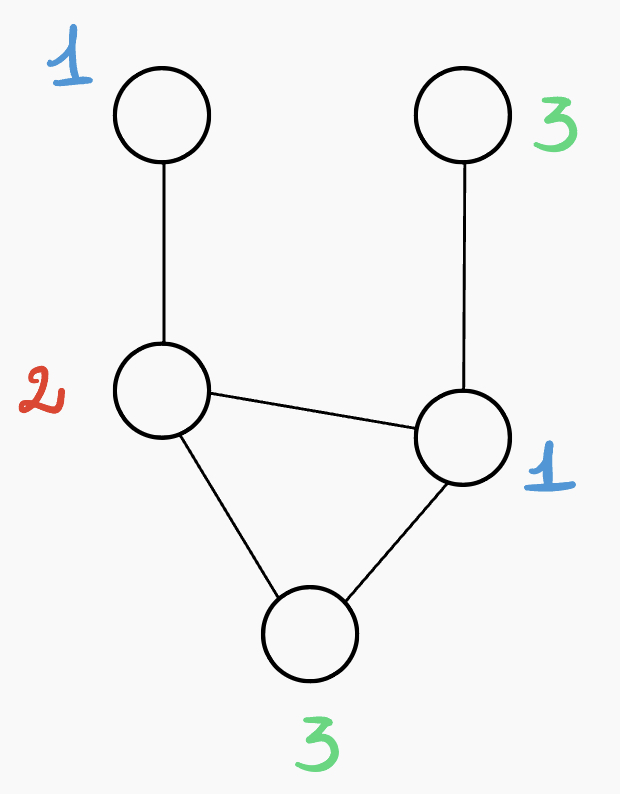
\includegraphics[width=0.3\linewidth]{graph_coloring_1.1.jpeg}
   				$\qquad$
   				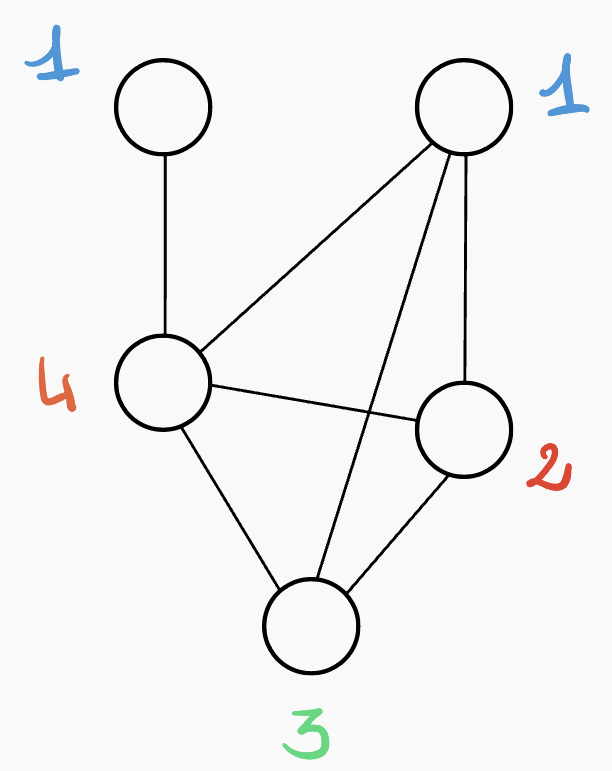
\includegraphics[width=0.3\linewidth]{graph_coloring_1.2.jpeg}
   			\end{center}
   		\end{exercise}
   		
   		\begin{exercise}{ 5: Graph 3-coloring}
   			\paragraph{Problem.} Prove that the following problem is in \textbf{NF}\\
   			$\mathcal{L} = \{\lfloor (G) \rfloor \; \vert \; G = (V, E)$ is an undirected graph and it contains a Hamiltonian cycle\}.\\
   			\paragraph{Solution.} A graph has an Hamiltonian cycle if it has a cycle that visits every vertex exactly once.
   			\begin{center}
   				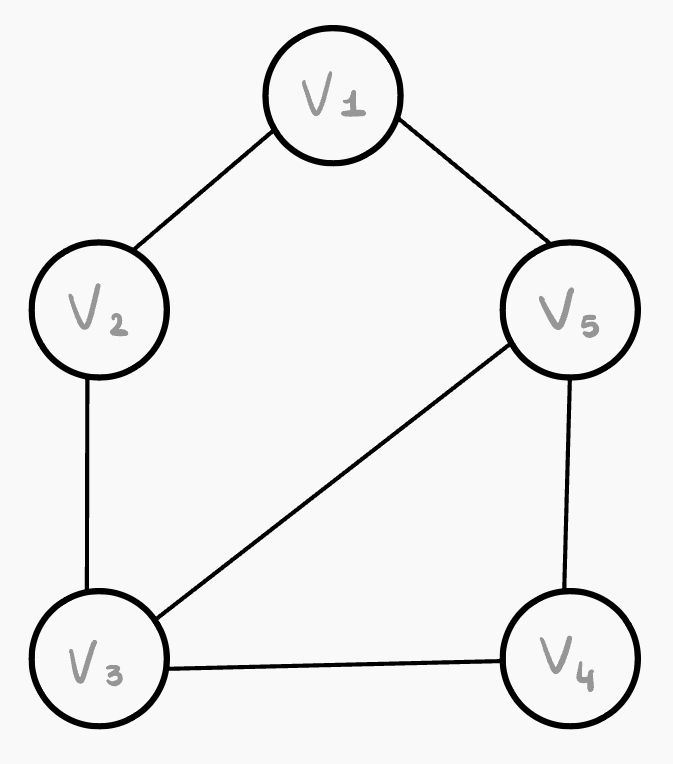
\includegraphics[width=0.26\linewidth]{graph_coloring_2.1.jpeg}
   			\end{center}
			$\mathbb{G} = (V, E)$
			\begin{itemize}
				\item \textbf{Certificate:} sequence $(v_1, \dots, v_n)$ with $n \leq |v| + 1$\\
				the certificate is polynomial in the length of the input.
				\item \textbf{Verifier:} input $\mathbb{G}, \mathbb{S} = (v_1, \dots, v_n)$
				\begin{algorithmic}
					\LComment{$O(|V|)$ steps since the length of the sequence is $\leq |V| + 1$}
					\For{$1 \leq i \leq n-1$}
    					\ForAll{$(v_i, v_{i+1})$}
    						\If {$(v_i, v_{i+1})$ is not in E}
    							\State return false
    						\EndIf
    					\EndFor
    				\EndFor
    				\LComment{initialize an array $A$ of size $|V|$ with $0$ everywhere $\rightarrow A[v] = 0$ for all $v$ in $V$}
    				\LComment{check that the sequence s does not contain a vertex twice from $v_1$ to $v_{n-1}$}
    				\For{$1 \leq i \leq n-1$} \Comment{$O(|V|)$}
    					\LComment{there is a vertex twice}
    					\If{$A[v_i] == 1$}
    						\State return false
    					\Else
   							\State $A[v_i] = 1$
   						\EndIf
   					\EndFor
   					\ForAll{$v$ in $V$}
   						\LComment{the sequence s does not visit all vertices in V}
    					\If{$A[v] == 0$} \Comment{$O(|V|)$}
   							\State return false
   						\EndIf
    				\EndFor
    				\If{$v_i == v_n$}
    					\State return true
    				\EndIf
				\end{algorithmic}
			\end{itemize}
     	\end{exercise}
\end{comment}


%%%%%%%%%%%%%%%%%%%%%%%%%%%%%%%%%%%%%%%%%%%%%%%%%%%%%%%%%%%%%%%%%%%%%%%%%%%%%%%%%
% Lecture 9 - 25.03.24
\begin{comment}
		\clearpage
   			\begin{pane}
   				$f: \{0, 1\}^* \rightarrow \{0,1\}^*$\\
   				$\mathcal{L} \subseteq \{0,1\}^*$
   				Given this problem, we could have all those possible outcomes:
   				\begin{center}
   					\begin{itemize}
   						\item undecidable
   						\item decidable
   						\item EXP
   						\item NP
   						\item P
   					\end{itemize}
   					\BoxedString{decidable $\subseteq$ \BoxedString{EXP $\subseteq$ \BoxedString{NP $\subseteq$ \BoxedString{P}}}}
   				\end{center}
   			\end{pane}
   			\begin{Theorem}{}{}
   				P $\subseteq$ NP $\subseteq$ EXP
   			\end{Theorem}
   			\begin{proof}
   				\mbox{}
   				\begin{enumerate}
   					\item We want to prove that P $\subseteq$ NP. Let us consider $\mathcal{L} \in$ NP. By the hypothesis, we know that there is a polynomial-time TM $\mathcal{N}$ which decides $\mathcal{L}$. We want to prove	 that $\mathcal{L}$ is in NP, namely that there are P and $\mathcal{M}$ (working in polynomial-time) such that:
   					$$\mathcal{L} = \{ x \in \{0,1\}^* \vert \exists y \in \{0,1\}^{P(|x|)}\;.\; \mathcal{M}(x,y) = 1 \} \qquad(*)$$
   					We can take P to be just 1. $\mathcal{M}$ can be a ``proxy" that returns 1 iff $\mathcal{N}(x) = 1$, on input $(x,y)$.
   					We want to be sure that $(*)$ holds.
   					\begin{align*}
   						\mathcal{L} &= \{x \in \{0,1\}^* \; \vert \; \mathcal{N}(x) = 1\} =\\
   						&= \{x \in \{0,1\}^* \; \vert \; \mathcal{N}(x,y) = 1 \text{ for some } y \in \{0,1\}^1\} =\\
   						&= ..
   					\end{align*}
   	  			\end{enumerate}
   				\begin{enumerate}
   					\setcounter{enumi}{1}
   					\item Suppose $\mathcal{L} \in$ NP. We want to prove ..\\
   					\textbf{input:} $x \in \{0,1\}^*$\\
   					\textbf{output:} $1 \text{ if } x \in \mathcal{L} \text{ and } 0 \text{ otherwise}$\\
   					\begin{algorithmic}
   						\ForAll {$y \in \{0,1\}^{P(|x|)}$} \Comment{$2^{P(|x|)}$}
   							\If {$\mathcal{M}(x,y) = 1$} \Comment{$O(q(|x|+|y|))$}
   								\State return 1 \Comment{$O(1)$}
   							\EndIf
   						\EndFor
   						\State return 0
   					\end{algorithmic}
   					The total amount of work performed by this algorithm is $O(2$ ..
   				\end{enumerate}
   			\end{proof}
   		
   		
   	\section{Between the feasible and the unfeasible}
   			\subsection{Reductions and complexity}
   			\mbox{}
   				
   			$\mathbb{R}$ is
   			\begin{itemize}
   				\item \uline{Reflexive} if $x \mathbb{R} x$ for every $x$.
   				\item \uline{Transitive} if $x \mathbb{R} y$ and $y \mathbb{R} z$ implies $x \mathbb{R} z$.
   			\end{itemize}
\end{comment}


%%%%%%%%%%%%%%%%%%%%%%%%%%%%%%%%%%%%%%%%%%%%%%%%%%%%%%%%%%%%%%%%%%%%%%%%%%%%%%%%%
% Lecture 11 - 08.04.24
\begin{comment}
		\clearpage
   		\begin{myproof}{NP-hardness of indset}
   			...\\
   			
   			The property we want to prove is that
   			$$C_1 \in \text{indset}$$
   			\textcolor{gray}{\hrule}
   			\begin{proof}
   				\mbox{}
   				\begin{itemize}
					\item Suppose that $C_1 \in 3SAT$. This means that there is an assignment $p: VAR \rightarrow \{ 0,1 \}$ such that $p \models C_i$ for every $i$.
					\item Each $l_i$ is part of a different clause (or column) so the edges panning columns are not a problem. Moreover it cannot be that two literals in the form $x, \neg x$ are part of the independent set, because if $C \models x$, $p \models \neg x$ then we have a contradiction.\\
					\item Suppose $(\mathbb{G}, \mathbb{K})$ has an independent set of cardinality grater or equal to $m$. The cardinality, in fact, must be $m$.
					\begin{itemize}
						\item .if $x$ is part of $X$, then $\rho(x) = 1$\\
						\item .if $\neg x$ is part of $X$, then $\rho(x) = 0$\\
						\item .if neither $x$ nor $\neg x$ are in $X$, then $\rho(x)$ can be anything.
					\end{itemize}
					My claim, then, is that $\rho$ makes the formula true, i.e. $\rho \models C_1 \dots C_m$. We have, indeed, built $\rho$ in such a way that it mimicks $X$, and $X$ spans all clauses $C_1, \dots, C_m$.
				\end{itemize}
			\end{proof}
   		\end{myproof}
   		\begin{myproof}{2SAT is in P}
   			\begin{proof}
   				We can see 2CNFS as directed graphs as follows:\\	
   			\end{proof}
   		\end{myproof}
   		\begin{exercise}{: SAT}
   			Consider the following problem:
   			
   		\end{exercise}
\end{comment}


%%%%%%%%%%%%%%%%%%%%%%%%%%%%%%%%%%%%%%%%%%%%%%%%%%%%%%%%%%%%%%%%%%%%%%%%%%%%%%%%%
% Lecture 12 - 15.04.24
\begin{comment}
	\clearpage
   	\section{A glimpse of computational learning theory}
   		\subsection{Is $\mathcal{A}_{BFP}$ (approximately) correct?}
   		\begin{Theorem}{}{}
   			\textit{For every distribution $\mathbf{D}$, for every $0<\epsilon<\frac{1}{2}$ and for every $0<\delta<\frac{1}{2}$,\\if $m\geq\frac{4}{\epsilon}\ln{\frac{4}{\delta}}$, then}
   			$$\operatorname*{Pr}_{D\sim\mathbf{D}^{m}}[error_\mathbf{D,T}(\mathcal{A}_{BFP}(T(D)) < \epsilon] > 1-\delta$$
   		\end{Theorem}
   		\begin{proof}
   			\mbox{}
   			\begin{itemize}
   				\item Let us first look at the expression $error_\mathbf{D,T}(\dots)$ we have in the thesis. It is actually true that
   				$$error_\mathbf{D,T}(\dots) = \operatorname*{Pr}_{x\sim\mathbf{D}}[x \in (R - T) \cup (T - R)]$$
   				where $R$ is the rectangle $\mathcal{A}_{BFP}(T(D))$ produced in output by our algorithm.
   				\item Since $R - T$ is empty, we na rewrite the above as follows:
   				$$error_\mathbf{D,T}(\dots) = \operatorname*{Pr}_{x\sim\mathbf{D}}[x \in T - R]$$
   				\item Let's take a look at $T - R$:
   				\begin{center}
   					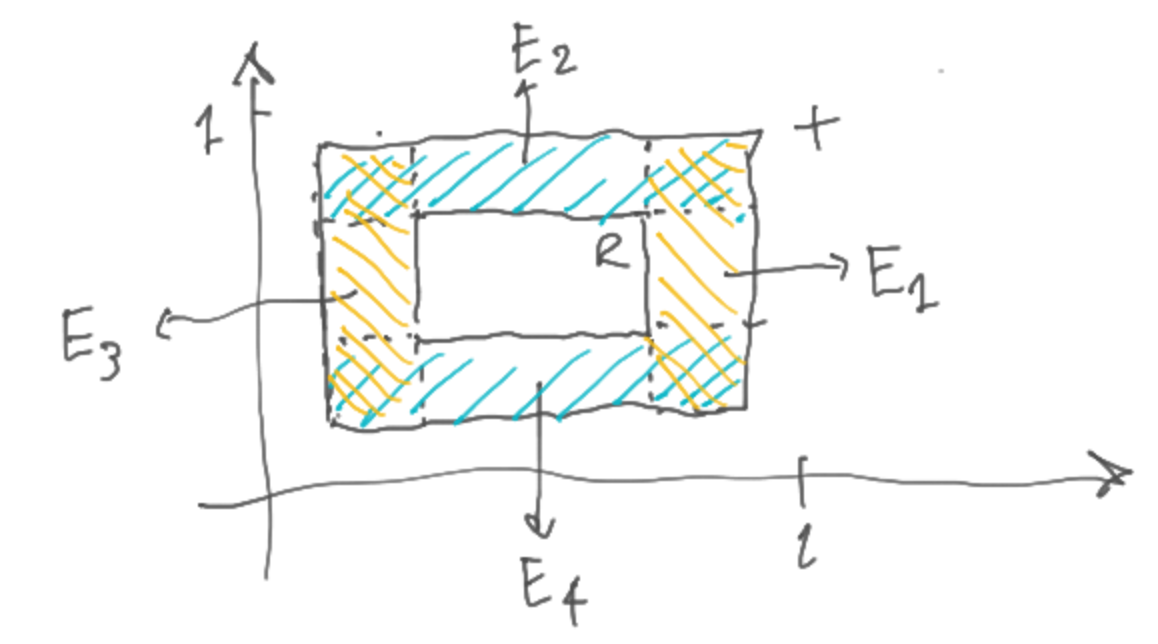
\includegraphics[width=0.5\linewidth]{proofs_computational_learning_theory_1}
   				\end{center}
   				\item Consider the probabilistic event ``$x \in E_i$". This holds in $x \sim \mathbf{D}$ precisely in those situations in which none of the training data are in $E_i$.
   				\item Let us consider other regions of the plane which are related to the $E_{is}$ but defined differently\\
   				\begin{minipage}[h]{0.49\linewidth}
   				\begin{center}
   					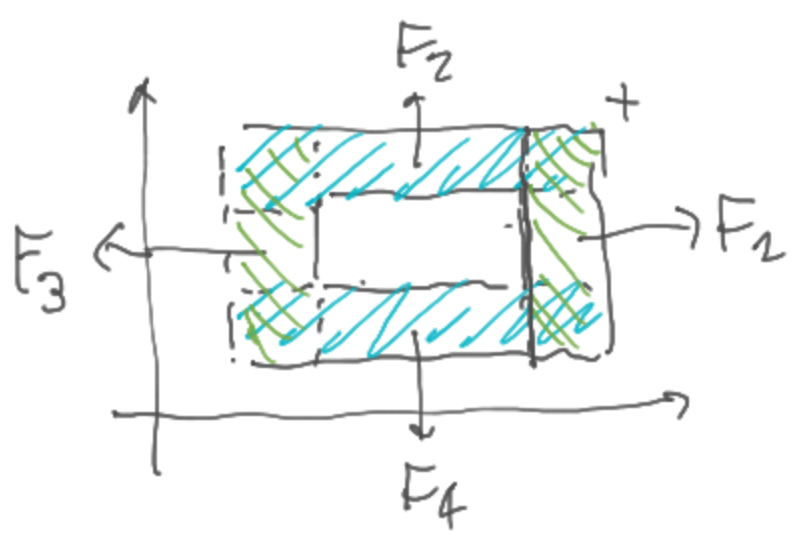
\includegraphics[width=0.8\linewidth]{proofs_computational_learning_theory_2}
   				\end{center}
   				\end{minipage}
				\hfill
				\begin{minipage}[t]{0.49\linewidth}
					$$\operatorname*{Pr}_{x\sim\mathbf{D}} (x \in F_i) = \frac{\epsilon}{4}$$
				\end{minipage}
   				\item Some easy probabilistic arguments lead us to
  				\begin{align*}
  					\text{\scriptsize\textcolor{gray}{{$\operatorname*{Pr}[A \cup B] \leq \operatorname*{Pr}[A]$}}} & \text{\scriptsize\textcolor{gray}{{$+ \operatorname*{Pr}[B]$}}}\\
  					\operatorname*{Pr}_{x\sim\mathbf{D}} [x \in E_i] < \frac{\epsilon}{4} \quad \Longrightarrow \quad &\operatorname*{Pr} [x \in T - R] < \epsilon\\
  					\quad \Longrightarrow \quad &error_\mathbf{T,D}(R) < \epsilon
  				\end{align*}
 			\end{itemize}
   		\end{proof}
   		We want now to prove another implication:
   		\begin{pane}
   			\begin{align*}
  				\text{``\textbf{Some red points in the}}\\
  				\text{\textbf{training data are in $F_i$}"}
  				& \quad \Longrightarrow \quad E_i \subseteq F_i\\
  				& \quad \Longrightarrow \quad \operatorname*{Pr}_{x\sim\mathbf{D}} (x \in E_i) < \frac{\epsilon}{4} + \ln{(e^{-\frac{\delta}{n}})^m}
  			\end{align*}
  			\vspace{0cm}
   		\end{pane}
  		\begin{proof}
  			\begin{align*}
   				m\geq(\ln{\frac{4}{\delta}})\cdot\frac{4}{\epsilon} & \quad \Longrightarrow \quad \frac{\epsilon \cdot m}{4}\geq \ln{\frac{4}{\delta}} \; \Rightarrow \; \ln{4}\\
   				& \quad \Longrightarrow \quad \\
   				& \quad \Longrightarrow \quad \operatorname*{Pr}\;(\forall i \; . \; \text{``\textit{some points in the training data occur in $F_i$}"})
   			\end{align*}
  		\end{proof}
   		\subsection{The general model - PAC concept classes}
   		\begin{Definition}{PAC learnability}{}
   			Let $\mathcal{C}$ be a concept class over the instance space $X$. We say that $\mathcal{C}$ is \textbf{PAC learnable} iff there is an algorithm $\mathcal{A}$ such that for every $c \in \mathcal{C}$, for every distribution $\mathbf{D}$, for every $0<\epsilon<\frac{1}{2}$ and for every $0<\delta<\frac{1}{2}$, then
   			$$\operatorname*{Pr}[error_{\mathbf{D},c}(\mathcal{A}(EX(c,\mathbf{D}),\epsilon,\delta)) < \epsilon] > 1 - \delta$$
   			where the probability is taken over the calls to $EX(c,\mathbf{D})$.
   		\end{Definition}
   		\begin{Definition}{Efficient PAC learnability}{}
   			If the time complexity of $\mathcal{A}$ is bounded by a polynomial in $\frac{1}{\epsilon}$ and $\frac{1}{\delta}$, we say that $\mathcal{C}$ is \textbf{efficiently PAC learnable}.\\
   			The complexity of $\mathcal{A}$ is measured taking into account the number of calls to $EX(c,\mathbf{D})$.
   		\end{Definition}
   		\begin{Corollary}{}{}
   			\textit{The concept-class of axis-aligned rectangles over $\mathbb{R}^2_{[0,1]}$ is efficiently PAC-learnable.}
   		\end{Corollary}
\end{comment}


%%%%%%%%%%%%%%%%%%%%%%%%%%%%%%%%%%%%%%%%%%%%%%%%%%%%%%%%%%%%%%%%%%%%%%%%%%%%%%%%%
% Lecture 12 - 15.04.24
\begin{comment}
		\subsection{Learning Conjunctions of Literals}
			$n=4$\\
			$(0010, 1) \rightarrow$ the formula is TRUE\\
			$(0100, 0) \rightarrow$ the formula is FALSE\\
			$(1111, 0) \rightarrow$ the formula is FALSE
			
		\begin{Theorem}{}{}
			\textit{The representation class of boolean conjunctions of literals is efficiently PAC learnable.}
		\end{Theorem}
		\begin{proof}
			\mbox{}
			
			One can use the algorithms we ...\\
			If the number of samples is at least
			$$(\ln{2n + \ln{\frac{1}{\delta}}}) \cdot \frac{2n}{\epsilon}$$
			We can prove that
			$$\operatorname*{Pr}_{D\sim D^m} (error(h)<\epsilon) < 1 - \delta$$
			The crux of the proof is ...
		\end{proof}
		
		\begin{Theorem}{}{}
			\textit{If $\mathbf{NP} \neq \mathbf{RP}$, then the representation class of 3-term DNFs is not efficiently PAC learnable.}
		\end{Theorem}
		\begin{proof}
			You can structure the proof as a reduction, namely you show that the following function is polytime computable.
			$$\alpha \in \{0,1\}^* \quad |\longrightarrow \quad S_\alpha$$
		\end{proof}
\end{comment}


%%%%%%%%%%%%%%%%%%%%%%%%%%%%%%%%%%%%%%%%%%%%%%%%%%%%%%%%%%%%%%%%%%%%%%%%%%%%%%%%%
% Lecture 14 - 23.04.24 (Exercitation)
\begin{comment}
		\begin{exercise}{: Closure properties of NP}
			\paragraph{Problem.} Prove that the class \textbf{NP} is closed under intersection and concatenation.\\
			
			\paragraph{Solution.}
			\mbox{}
			 
			\begin{algorithmic}
				\State define $\mathcal{A}(x,y)$
				\If {$y==y_1 \# y_2$}
    				\State return 0
    			\EndIf
			\end{algorithmic}
			Define polynomials $p,q: \; \mathbb{N}\rightarrow\mathbb{N}$ as
			$$p(n) = p_1(n) + p_2(n) + 1 \quad \textcolor{gray}{(y = y_1 \# y_2)}$$
			$$q(n) = q_1(n) + q_2(n)$$
			Define $\mathcal{L} = \{x \in \{0,1\}^* \mid ... \}$
			\begin{enumerate}
				\item $\mathcal{L}$
				\item $\mathcal{L}\subseteq\mathcal{L}_1\cap\mathcal{L}_1$ the proof is similar.
			\end{enumerate}
		\end{exercise}
		\begin{pane}
			$\mathcal{L} = \{0^n 2^n \mid n \in \mathbb{N} \}$\\
			$\epsilon, \; 01, \; 0011, \; 000111$\\
			$\in \mathcal{L}^+$\\
			$\epsilon, \; 00011101$\\
			$01 \; 01 \; 0011$
		\end{pane}
		\vspace{0.5cm}
		\begin{exercise}{: Vertex cover}
			\paragraph{Problem.} Assuming that {\footnotesize INDSET} is \textbf{NP}-complete, show that {\footnotesize VERTEXCOVER} is also \textbf{NP}-complete.\\
			\paragraph{Solution.}
			\mbox{}
			\vspace{0.2cm}
			
			\begin{enumerate}
				\item {\footnotesize VERTEXCOVER} is in NP\\
				
				certificate $S \subseteq V$\\
				verifier input $G = (V, E) \quad k \quad S$
				\begin{algorithmic}
					\If {$|S| > k$}
						\State return false
					\EndIf
					\LComment {initialize a empty queue $q$}
					\State queue $q$
					\ForAll{$(u,v)$ in E}
						\State $q$ append $(u.v)$
					\EndFor
					\While {!q empty()}
						\ForAll{$w$ in $S$}
							\State $(u,v) \leftarrow q \; \cdot$ dequeue()
							\If{$!u == w$ and $!v == u$}
								\State $a \; \cdot$ append($u,v$)
							\EndIf
						\EndFor
					\EndWhile
				\end{algorithmic}
				
				\item {\footnotesize INDSET} $\leq_p$ {\footnotesize VERTEXCOVER}\\
				
				$G = (V,E),\;k \quad \longmapsto \quad G', k'$\\
				such that $G$ has an independent set of size at least $k$ iff $G'$ has a vertex cover of size at most $k'$.\\
				We show that $G$ has independent set of size at least $k$ iff $G' = G$ has vertex cover of size at most $\underbrace{|V| - k}_{k'}$.\\
				
				\begin{align*}
					S \subseteq V \text{ is an independent set }&\text{iff} \; \forall(u,v) \text{ in E}, \; u \notin S \text{ or } v \notin S \qquad \qquad \qquad \qquad \\
					&\text{iff} 
				\end{align*}
			\end{enumerate}
		\end{exercise}
		\begin{exercise}{: Graph 2-coloring problem}
			\paragraph{Problem.}
			\begin{itemize}
				\item Recall: an undirected graph $G = (V,E)$ is $k$\textit{-colorable} if there exists a function
				$$color: \; V\rightarrow(1,\dots,k)$$
				such that for all edges $(u,v) \in E, \; color(u) \neq color(v)$.
				\item Show that the 2-coloring problem {\footnotesize 2COL} is in \textbf{P}:
				\begin{center}
					$\quad$\textbf{input}$\quad$ an undirected graph $G = (V,E)$\\
					$\;$\textbf{output}$\quad$ $1$ if $G$ is 2-colorable, $0$ otherwise
				\end{center}
			\end{itemize}
			\textcolor{gray}{\hrule}
			\paragraph{Solution.}
			\mbox{}
			
			\begin{algorithmic}
				\State input graph $G = (V,E)$
				\State $m \leftarrow |V|$
				\If{$m == 0$}
					\State return 1
				\EndIf
				\State int $A[n]$ \Comment{array of colors of size $n$}
				\ForAll{$1 \leq i \leq n$}
					\State $A[i] = 0$
				\EndFor
			\end{algorithmic}
			
			
			\textcolor{red}{**aggiungere disegno iPad**}
		\end{exercise}
		\begin{exercise}{: Graph 3-coloring problem}
			\paragraph{Problem.}
			\begin{itemize}
				\item Using the fact that \textbf{3SAT} is \textbf{NP}-complete, show that the 3-coloring problem {\footnotesize 3COL} is also \textbf{NP}-complete.
				\begin{center}
					$\quad$\textbf{input}$\quad$ an undirected graph $G = (V,E)$\\
					$\;$\textbf{output}$\quad$ $1$ if $G$ is 3-colorable, $0$ otherwise
				\end{center}
			\end{itemize}
			\textcolor{gray}{\hrule}
			\paragraph{Solution.}
			\mbox{}
			
			\begin{enumerate}
				\item {\footnotesize 3COL} in \textbf{NP} (previous exercise session)
				\item {\footnotesize 3COL} is \textbf{NP}-Hard by showing that {\footnotesize 3SAT}
			\end{enumerate}
		\end{exercise}
\end{comment}






	\cleardoublepage
	\addcontentsline{toc}{section}{References} 
	\begin{thebibliography}{9}
		\bibitem{arora2007}
			Sanjeev Arora and Boaz Barak. \emph{Computational Complexity: A Modern Approach}. Cambridge University Press. 2007.
		\bibitem{papadimitriou1994}
			Christos Papadimitriou. \emph{Computational Complexity}. Addison-Wesley. 1994.
		\bibitem{shalev-shwartz2014}
			Shai Shalev-Shwartz and Shai Ben-David. \emph{Understanding Machine Learning: from Theory to Algorithms}. Cambridge University Press. 2014.
		\bibitem{kearns1994}
			Michael Kearns and Umesh Vazirani. \emph{An Introduction to Computational Learning Theory}. The MIT Press. 1994.
	\end{thebibliography}


	\appendix
	\newpage
	\section{Suggested books}
		\subsection*{To fill any gap:}
			\begin{figure}[h]
   				\setlength{\fboxsep}{0pt}
   				\setlength{\fboxrule}{0.7pt}
   				\fcolorbox{black}{white}{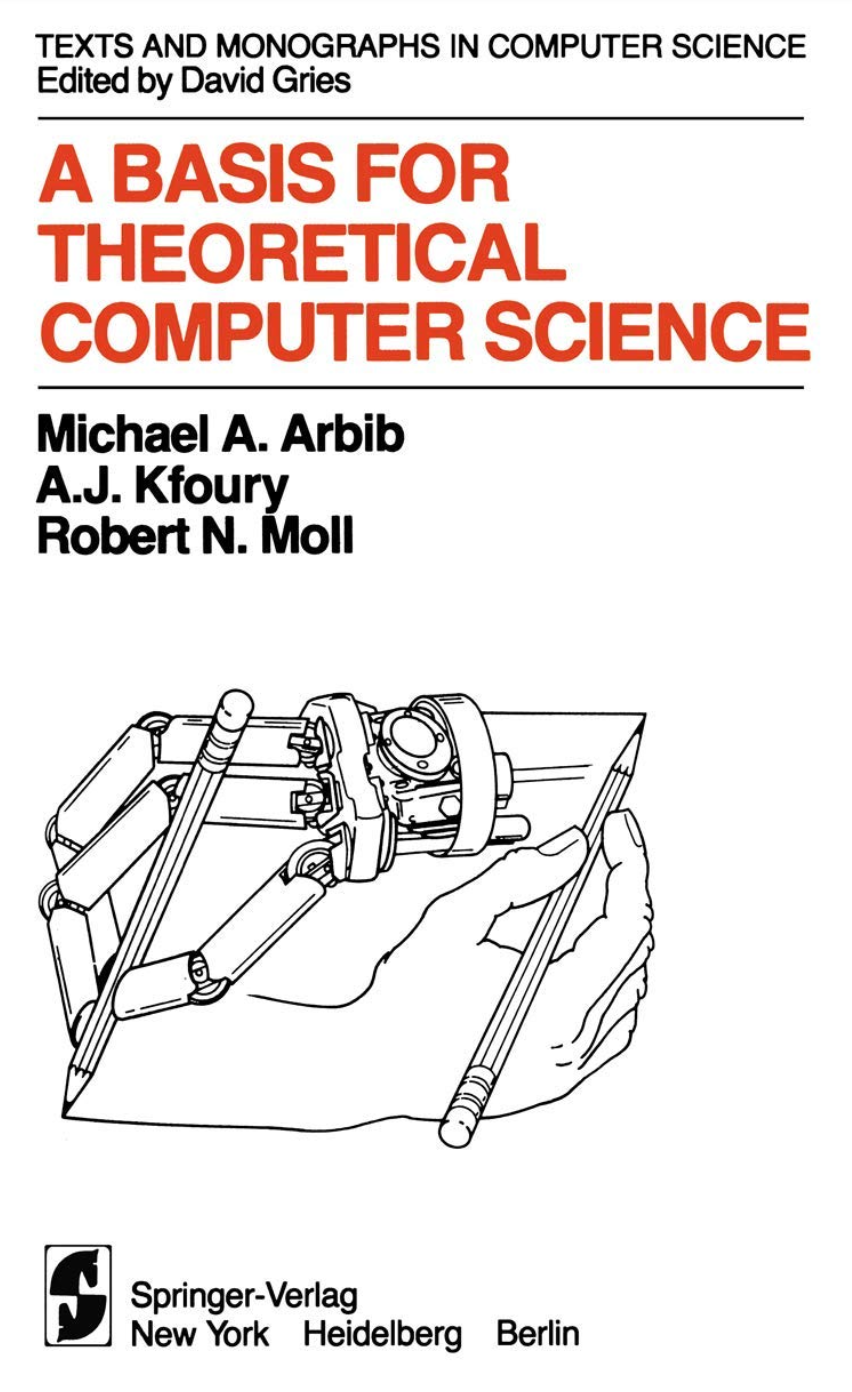
\includegraphics[height=0.2\textwidth]{book1}}
			\end{figure}
		
		\subsection*{References on ``Positive" Algorithmics:}
			\begin{figure}[h]
   				\setlength{\fboxsep}{0pt}
   				\setlength{\fboxrule}{0.7pt}
   				\fcolorbox{black}{white}{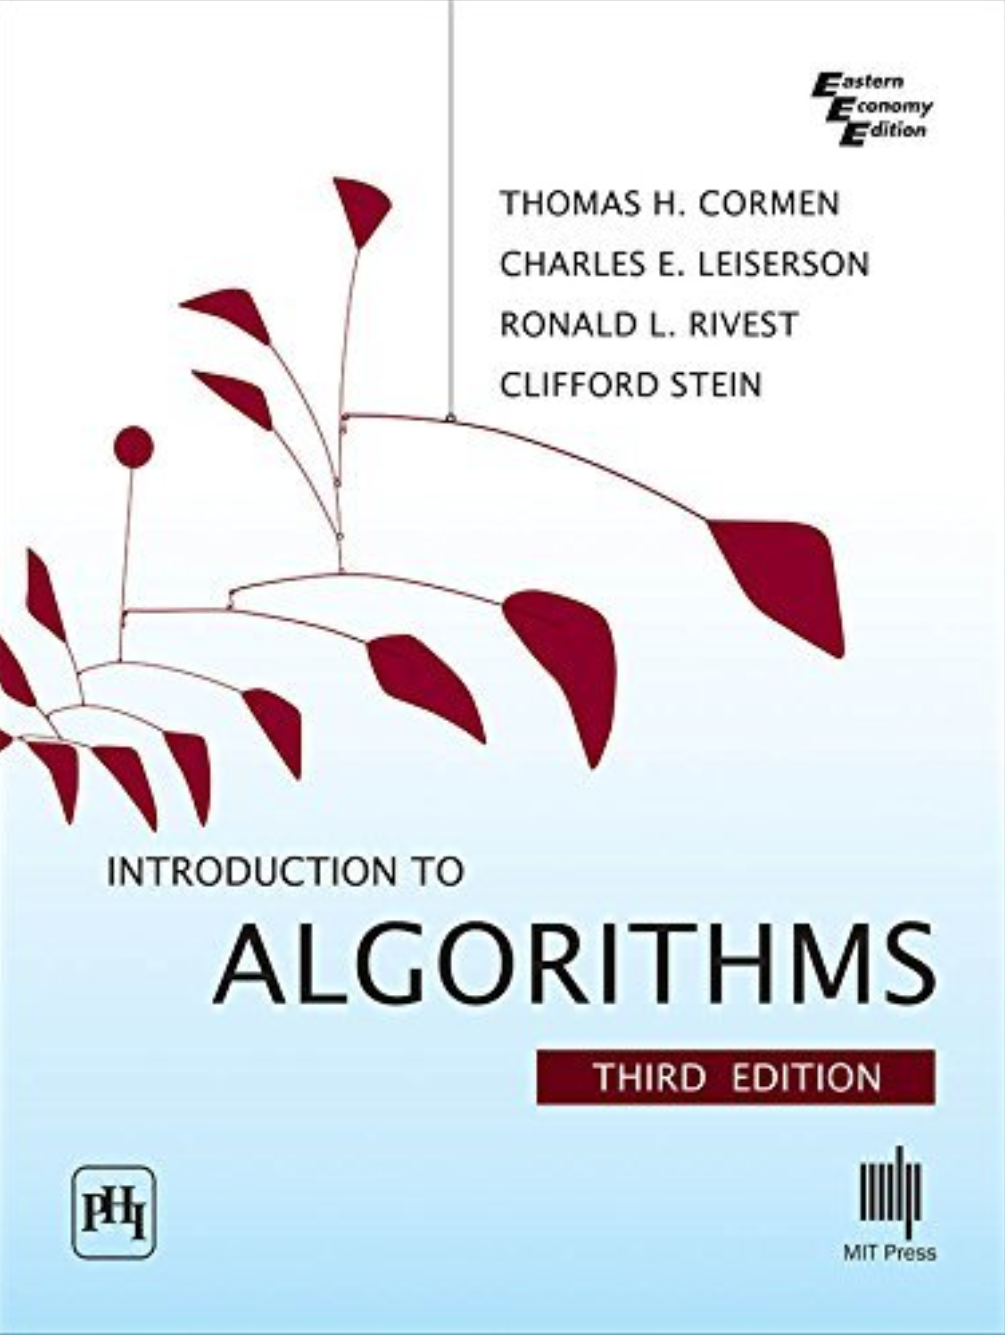
\includegraphics[height=0.2\textwidth]{book2}}
   				\setlength{\fboxsep}{0pt}
   				\setlength{\fboxrule}{0.7pt}
   				\fcolorbox{black}{white}{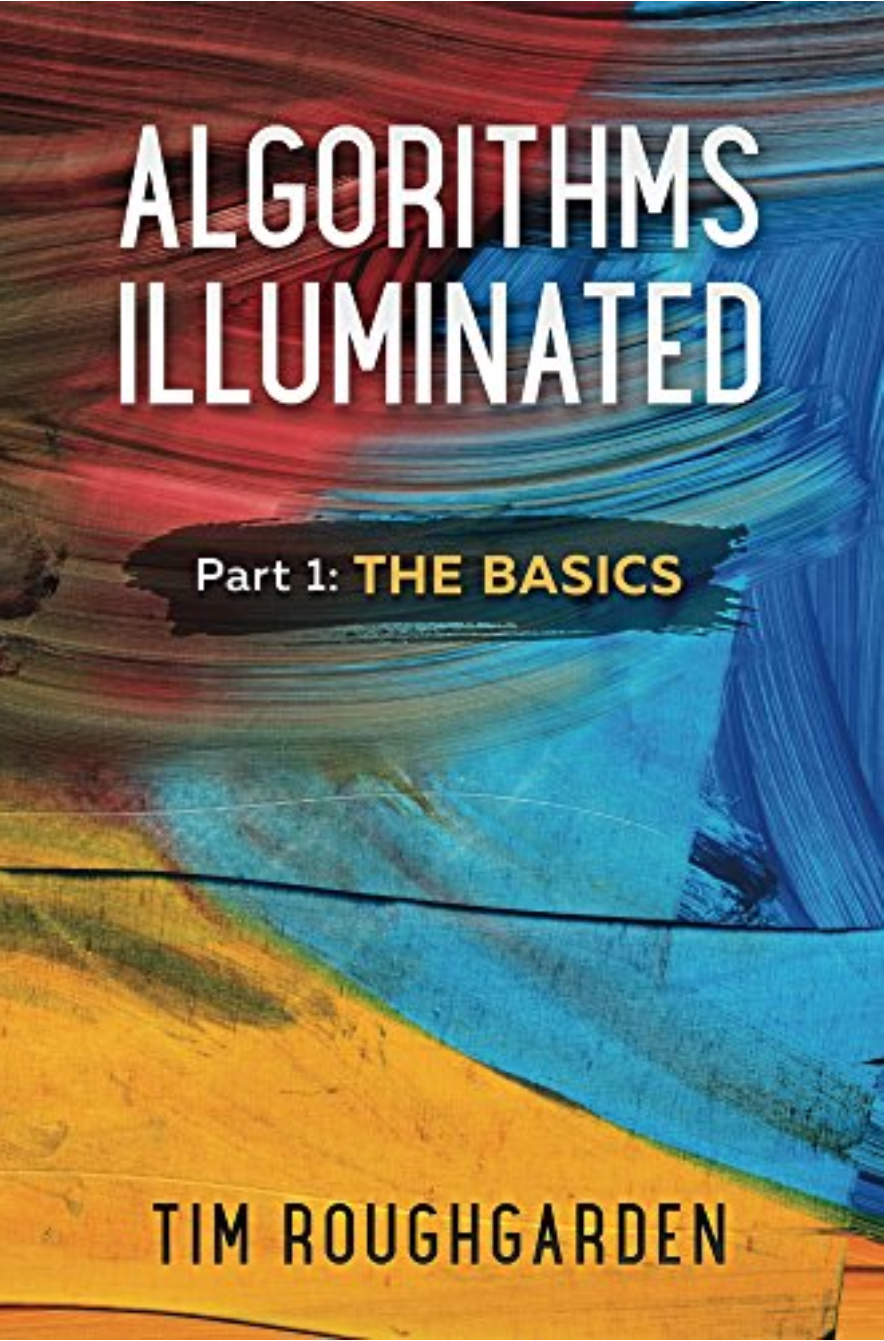
\includegraphics[height=0.2\textwidth]{book3}}
			\end{figure}
\end{document}

